\section{Work schedule and flow}\label{sec:workscheduleandflow}

In this section we will discuss the work schedule we put together and how we managed to follow that schedule. We will also go into the methodology we decided to use to aid us during the project and how that influenced the project. As a part of that we will show the burndown chart for the project as a whole and discuss all of the sprints that we finished while working on the project.

\subsection{Initial plan}

Our work schedule was split into two different phases. The first was during the 12 week semester from the 17th of August to November the 11th. Our schedule during that period was influenced by classes and course work in other courses. During the 3 week semester from the 26th of November to December the 16th this project was our only concern so we could dedicate most of our time to it. 

\subsubsection{Schedule for the 12 week semester}
  This table gives a detailed view of the hours we scheduled to work on the project during the 12 week term. This was the minimum amount of hours we pledged to dedicate to the project during the term. The difference in hours spent on the project for team members during this phase can be explained by a more favorable schedule in other courses for Jóhann. 

  \noindent
  \addvbuffer[12pt 12pt]{\begin{tabular} {| r | c | c | c | c | c | c | c |}
    \rowcolor{LightSteelBlue}
    \hline  & Mon & Tue & Wed & Thu & Fri & Sat & Sun\\ 
    \hline Hjalti & 16:00-18:00 & 16:00-18:00 & - & 12:00-15:30 & 10:00-14:00 & -  & - \\
    \hline  & - & - & - & - & 16:00-18:00 & - & - \\
    \hline Total & 2:00 & 2:00 & - & 3:30 & 6:00 & - & - \\
    \rowcolor{LightSteelBlue}
    \hline  &  Mon & Tue & Wed & Thu & Fri & Sat & Sun\\ 
    \hline Jóhann & 16:00-18:00 & 16:00-18:00 & - & 9:30-15:30 & 10:00-14:00 & -  & - \\
    \hline  & - & - & - & - & 16:00-18:00 & - & - \\
    \hline Total & 2:00 & 2:00 & - & 6:00 & 6:00 & - & - \\
    \hline
  \end{tabular}}

  \noindent This table sums up the total hours for the 12 week term.  
  
  \noindent
  \addvbuffer[12pt 12pt]{\begin{tabular} {| r |  c | c |}
  \hline & Hjalti & Jóhann\\
  \hline Total per week & 13.5 hours & 16 hours \\
  \hline Total for the semester & 162 hours & 192 hours \\
  \hline Total combined & \multicolumn{2}{c |}{354 hours} \\ 
  \hline
	
  \end{tabular}} 
  
\subsubsection{Schedule for the 3 week semester}
  This table shows the schedule for the 3 week term. The hours are the minimum commitment both team members made during this time.

  \noindent
  \addvbuffer[12pt 12pt]{\begin{tabular} {| r | c | c | c | c | c | c | c |}
    \rowcolor{LightSteelBlue}
    \hline  & Mon & Tue & Wed & Thu & Fri & Sat & Sun\\ 
    \hline Hjalti & 9:00-17:00 & 9:00-17:00 & 9:00-17:00 & 9:00-17:00 & 9:00-17:00 & 10:00-15:00  & 10:00-15:00 \\
    \hline Total & 8:00 & 8:00 & 8:00 & 8:00 & 8:00 & 5:00 & 5:00 \\
    \rowcolor{LightSteelBlue}
    \hline  &  Mon & Tue & Wed & Thu & Fri & Sat & Sun\\ 
    \hline Jóhann & 9:00-17:00 & 9:00-17:00 & 9:00-17:00 & 9:00-17:00 & 9:00-17:00 & 10:00-15:00  & 10:00-15:00 \\
    \hline Total & 8:00 & 8:00 & 8:00 & 8:00 & 8:00 & 5:00 & 5:00\\
    \hline
  \end{tabular}}

  \noindent This last table summarizes the total amount of hours we scheduled to spend on the project.
  
  \noindent
  \addvbuffer[12pt 12pt]{\begin{tabular} {| r |  c | c |}
  \hline & Hjalti &  Jóhann\\
  \hline Total per week & 50 hours & 50 hours \\
  \hline Total for the semester & 150 hours & 150 hours \\
  \hline Total for the previous semester & 162 hours & 192 hours \\
  \hline Total for the project & 312 hours & 342 hours \\
  \hline Total for the project combined & \multicolumn{2}{c |}{654 hours} \\ 
  \hline
  \end{tabular}}


\subsection{Methodology}
For this project we utilized the Scrum methodology to help us document and organize the project and its progress. The appointed Scrum Master was Jóhann and the Product Owner was Hjalti. Pétur Örn Þórarinsson, a lead game designer at CCP, served as our Project Manager. Since the team only consisted of two people, the Scrum Master and Product Owner made up the the whole team. The project consisted of seven, two week long sprints, with the work divided so that the team could direct enough attention towards other courses, as well as work on the project.

Daily Scrum meetings were held at CCP headquarters every work day. During the three week term they took place at 11:30 AM, but they were held at various times of the day during the 12 week term, as the team wasn't always present throughout the day. We chose Scrum because it gave us good documentation on the team's progress and it gave us an indication of what we could achieve according to our velocity. With each iteration we could track what was going well and what needed improving. Scrum gave us the platform to review and improve on our process during each iteration.

\subsection{Progress during the project}

\subsubsection{Actual hours spent}

The following charts show the hours spent by the team members individually and collectively during the 12 week term. Both team members spent more than the scheduled time on the project, Hjalti by 18 hours and Jóhann by 9 hours. The team did hoe

\begin{figure}[H]
  \centering
  \graphicspath{ {./graphics/} }
  \centerline{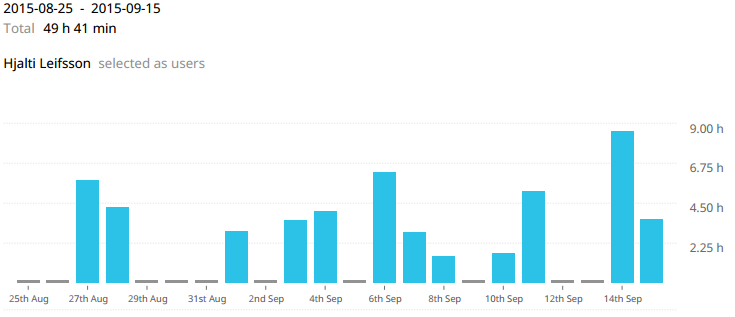
\includegraphics[scale=0.43]{hjalti.png}}
  \caption{\label{fig:hjalti}Total hours for Hjalti during the 12 week term}
\end{figure}

\begin{figure}[H]
  \centering
  \graphicspath{ {./graphics/} }
  \centerline{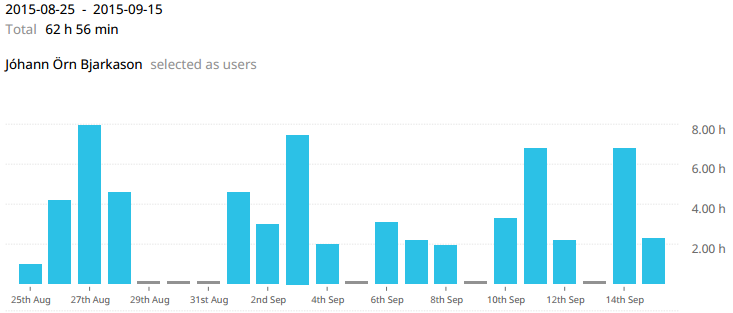
\includegraphics[scale=0.43]{johann.png}}
  \caption{\label{fig:johann}Total hours for Jóhann during the 12 week term}
\end{figure}

\begin{figure}[H]
  \centering
  \graphicspath{ {./graphics/} }
  \centerline{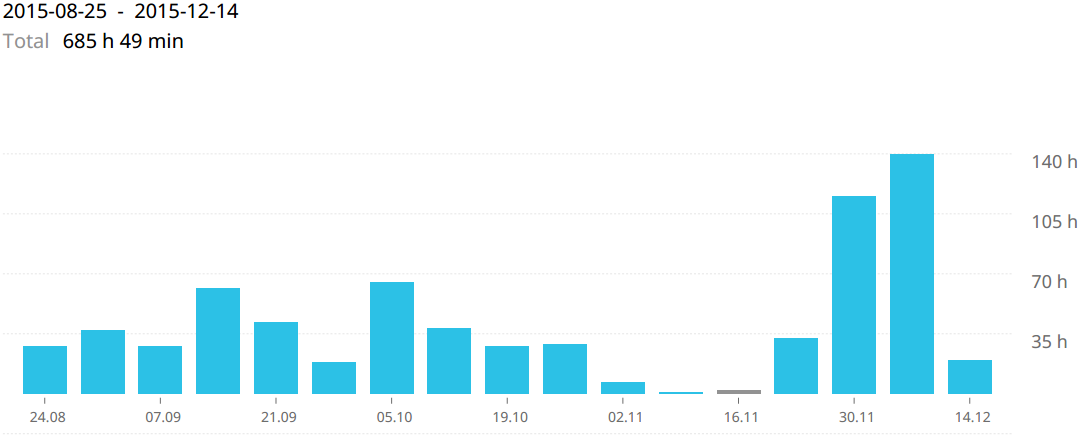
\includegraphics[scale=0.43]{total.png}}
  \caption{\label{fig:total}Total hours for the team during the 12 week term}
\end{figure}

TODO: Insert images from toggl of hours spent once work is done.

\subsubsection{Project burndown chart}

TODO: Insert a burndown chart once the final sprint is done.

\subsubsection{Sprint summary}

\subsection{Schedule summary}